%!TEX root = Vorlage_Buch.tex
\chapter{Beilagen und Snacks}\label{Chapter5}
\lettrine[lines=3]{BBQ}{bedeutet für mich} nicht nur Fleisch oder 'ne Rote im Brötchen. BBQ ist kochen und im Idealfall auch genießen im 
Freien. Fast alles was in der Küche im Haus zubereitet werden kann, kann auch in der Außenküche zubereitet werden.  Deshalb werde ich 
hier auch einige Rezepte vorstellen die von Oma gekocht wurden, bevor es jemanden gab der Barbecue (/ˈbɑː.bɪ.kjuː/)  aussprechen konnte.

Unter dem Punkt "`Ä Gosch voll"' werden wir Rezepte für kleine Happen kennenlernen.  Diese Häppchen sind mundgerecht und können als Amuse Gueule, 
zwischen den Gängen, als Dessert oder einfach als Fingerfood gereicht werden. In diesen Happen wird alles verpackt, das benötigt wird um Kleines ganz groß werde zu 
lassen. Also gehen wir es an.  

\section{Ä Gosch voll,}
besser beschreiben kann man die Kleinigkeiten nicht. Es ist wie im wirklichen Leben, die kleinen Dinge machen die meiste Arbeit, sorgen aber auch für den Größten 
Wow-Effekt. Daher bitte ein wenig Zeit einplanen, oder so viel möglich am Vortag vorbereiten. 

\subsection{Tiroler Schlutzkrapfen}

Schlutzkrapfen sind eine Nudelspezialität aus Tirol und werden aus einer 
Mischung von Roggen- und Weizenmehl hergestellt. Der Name leitet sich von 
"`Schluzen"' 
ab, was soviel wie Rutschen oder Gleiten bedeutet.

\paragraph{Geräte}

\begin{itemize}[noitemsep]
	\item Teigmaschine oder Hände
	\item Nudelmaschine
	\item Holzkohlegrill, Gasgrill oder Keramikgrill
\end{itemize}

\paragraph{Zutaten für die Schlutzkrapfen}

\begin{itemize}[noitemsep]
	\item 125 g Weizenmehl (hier Type 405)
	\item 125 g Roggenmehl (hier Type 997)
	\item 2 Eier
	\item 30 g Butter
	\item 2 L Wasser
	\item 1 TL Salz (hier Himalaya Salz)
\end{itemize}

\paragraph{Zubereitung}

Die beiden Mehlsorten mit dem Salz in einer Schüssel mischen. Die Butter zerlassen und mit den Eiern, dem Wasser hinzugeben. Das 
ganze mit der Küchenmaschine oder den Händen zu einem glatten Teig kneten. In ein Küchentuch einschlagen und 30 Minuten ruhen 
lassen.

\paragraph{Zutaten für die Füllung}

\begin{itemize}[noitemsep]
	\item 400 g vorwiegend festkochende Kartoffeln
	\item 1 Bund Minze
	\item 250 g Frischkäse
	\item 2 Knoblauchzehen
	\item Salz
	\item Cayennepfeffer
\end{itemize}

\paragraph{Zubereitung}

Kartoffeln ca. 25 Minuten kochen, abkühlen lassen und pellen. Die Kartoffeln noch warm durch eine Kartoffel- oder Spätzlepresse 
pressen und auskühlen lassen. Die Minze waschen, trocken schütteln und fein schneiden. Die Knoblauchzehen Schälen und sehr fein 
hacken, nicht pressen da sie bitter werden. Die Minze, den Knoblauch und 250 g Frischkäse zu den Kartoffeln geben, alles durchmischen 
und mit Salz und Cayennepfeffer abschmecken.

\paragraph{Finale Zubereitung der Schlutzkrapfen}

Den Nudelteig auf 2-3mm Stärke ausrollen und mit einem runden Ausstecher oder einem Glas ca. 8 cm durchmessende Kreise 
ausstechen. Diese mit der Kartoffelfüllung füllen, auf einer Seite benetzen, zusammenklappen und die Ränder mit den Fingern unter 
Druck verschließen.

Die "`Schlutzer"' in Salzwasser 3-4 Minuten leicht köcheln lassen. Die Teigtaschen auf gewässerte Holzspiese spießen und bei 
indirekter Hitze bei ca. 180 °C grillen, bis sie leicht gebräunt und ein wenig knusprig sind. Auf einem kleinen Teller oder Gourmetlöffel 
anrichten und mit Orangen-Chili-Butter (Rezept siehe 
Kapitel~\ref{Chapter6} \vref{OrangenChili}) beträufeln. Ein unglaubliches Geschmackserlebnis erwartet euch.

\subsection{Albóndigas}

Die Herkunft der Albóndigas en salsa, der spanischen Hackbällchen-Tapa lässt sich den arabischen Mauren zuschreiben. Sie brachten 
die al-búnduqa (arabisch für die Kugel) im 13. Jahrhundert nach Spanien. Im Morgenland wurden die Bällchen traditionell noch aus Lamm 
gerollt. In anderen Ländern kamen mit der Zeit Varianten aus Rind, Schwein, Wild, Geflügel oder Fisch dazu. Ich verwende gemischtes 
Hackfleisch aus Rind \& Schwein, um die Vorzüge der zwei Fleischsorten zu vereinigen. Das Rinderhack sorgt für einen kernigen Biss 
währen das fettere Schweinehack die Hackfleischbällchen saftig werden lässt.

\paragraph{Geräte}

\begin{itemize}[noitemsep]
	\item Holzkohlegrill, Gasgrill oder Keramikgrill
\end{itemize}

\paragraph{Zutaten}

\begin{itemize}[noitemsep]
	\item 400 g gemischtes Hackfleisch
	\item 1 kleine Zwiebel
	\item 1 Knoblauchzehe
	\item 1 TL Pimenton picante (Räucherpaprika)
	\item 1 TL Cumin geröstet und geschrotet
	\item 1 EL glatte Petersilie
	\item 1 Ei, Größe M
	\item 1 kleine Tasse Panko (60 g), trockenes Brot oder Semmelbrösel
	\item Salz, Pfeffer, Muskatnuss
	\item  Anschovis, gesalzen (nach Geschmack), die Anchovis können auch weggelassen werden
	\item 1 Prise Zimt
	\item 1/2 Kaschmir-Chili-Pulver
\end{itemize}

\paragraph{Zubereitung}

Den Grill mit einer direkten und indirekten Zone vorbereiten und auf eine Temperatur von 170°C bis 200°C einstellen.

Zwiebel und Knoblauch möglichst fein würfeln. Petersilie fein hacken. Cumin ohne Fett im Pfännchen anrösten und in der Gewürzmühle 
oder im Mörser grob mahlen. Die Anchovis ebenfalls hacken, werden keine Anchovis verwendet muss die Masse ein wenig stärker 
gesalzen werden. Altbackenes Brot klein schneiden und fein zerbröseln. Panko oder Semmelbrösel einfach direkt verwenden.

Saubere Hände anfeuchten und das Hackfleisch mit den geschnittenen Zutaten, Ei, Panko und den Gewürzen gründlich kneten. Zu 
kleinen Bällchen von ca. 4 cm Durchmesser rollen.
Die Bällchen auf gewässerte Holzspieße spießen und auf dem Grill bei direkter Hitze scharf angrillen und auf der indirekten Zone gar 
ziehen. Die Bällchen auf einem Gourmetlöffel oder einem kleinen Teller mit der Salsa de las Albóndigas (Rezept siehe 
Kapitel~\ref{Chapter6} \vref{SalsaAlbondigas}) anrichten und mit gehackter Petersilie bestreuen.

\subsection{Wachtelspiegelei auf marinierter Wachtelbrust}

\paragraph{Geräte}

\begin{itemize}[noitemsep]
	\item Gasgrill mit Plancha
\end{itemize}
	
\paragraph{Zutaten}

\begin{itemize}[noitemsep]
	\item 1 Wachtelbrüstle/ Person
	\item 1 Wachtelei/ Person
	\item Saft von einer Zitrone nach Bedarf
	\item Salz
	\item Pfeffer
	\item 1 Zweig Bio-Lavendel
	\item Wasser nach Bedarf
\end{itemize}

Die Wachtelbrüstchen über Nacht mit einer Marinade aus Zitronensaft, Bio-Lavendel und Wasser marinieren. Die Brüstchen trocken tupfen, mit Salz und Pfeffer würzen und  auf der Plancha bei ca. 200°C anbraten. Parallel dazu die Wachtelspiegeleier zubereiten. Alles auf einem Gourmetlöffel anrichten und mit ein wenig Lavendel garnieren.

\subsection{ Gegrillte Wachtelkeulen mit Chili-Butter }

\paragraph{Geräte}

\begin{itemize}[noitemsep]
	\item Gasgrill mit Plancha
\end{itemize}

\paragraph{Zutaten}

\begin{itemize}[noitemsep]
	\item 1 Wachtelkeulen/ Person
	\item Uwe's mediterrane Kräuterbutter (Rezept siehe~\vref{Kräuterbutter})
	\item Salz
	\item Pfeffer
	\item Geklärte Butter
	\item Pulver vom Kaschmir-Chili
\end{itemize}

Die Wachtelkeulen mit Kräuterbutter einreiben und die Kräuterbutter auch unter der Haut verteilen. Die Keulen werden auf der Plancha scharf angegrillt bis sich Röststoffe bilden, danach auf der indirekten Zone fertig gegart. Die geklärte Butter auf schwacher Hitze schmelzen und das Chili-Pulver einrühren. Das Pulver der Kaschmir-Chilis sorgt für eine tolle rote Färbung und hat einen guten  Geschmack bei moderater Schärfe. Die Keulen auf einem kleinen Teller anrichten und mit der Chili-Butter beträufeln.

\subsection{Jakobsmuschel an Orangenmayonnaise}

\paragraph{Geräte}

\begin{itemize}
	\item Gasgrill mit Plancha
\end{itemize}

\paragraph{Zutaten}

\begin{itemize}[noitemsep]
	\item 6 Jakobsmuscheln
	\item 6 Chicorée-Blätter
	\item Uwe's leckere Orangenmayonnaise (Rezept siehe 
	Kapitel~\ref{Chapter6} \vref{Orangenmayo})
	\item Zitronensaft
	\item Salz \& Pfeffer
	\item 50 g geklärte Butter
	\item 12 Blätter von der marokkanischen Minze
\end{itemize}

\paragraph{Zubereitung}

Gasgrill auf ca. 200°C aufheizen. Die geklärte Butter in einer kleinen Kasserolle erwärmen. 6 Blätter der Minze zugeben um die Butter zu aromatisieren. Die Jakobsmuscheln mit Zitronensaft beträufeln, mit Salz und Pfeffer würzen und auf die Plancha legen. Unter dessen die Chicorée-Blätter waschen und mit  Küchenpapier trocken tupfen. Ein Tupfer der Mayonnaise mit einer Dosierflasche auf die Chicorée-Blätter aufbringen. Die Jakobsmuscheln wenden sobald sie eine bräunliche Farbe angenommen haben und braten bis sie leicht gebräunt und in der Mitte noch glasig sind. Auf den Chicorée-Blättern anrichten, mit der aromatisierten, geklärten Butter beträufeln und mit einem Blatt der Minze garnieren.
\newpage

\subsection{Frühstück}

Das Frühstück werde ich hier unterbringen, da zu wenige Rezepte für ein eigenes Kapitel in dieses Buch Einzug finden.
Das Frühstück besteht aus Kartoffelpuffer, Spiegeleier, Bratwürste und gegrillten Tomaten.

\paragraph{Geräte}

\begin{itemize}[noitemsep]
	\item Gasgrill mit Plancha
\end{itemize}

\paragraph{Zutaten}

\begin{itemize}[noitemsep]
	\item 1,5 kg Kartoffeln
	\item 1 Gemüsezwiebel
	\item ca. 3 EL Mehl
	\item 2 Eier (für die Kartoffelpuffer)
	\item Neutrales Öl
	\item Salz \& Pfeffer
	\item 4 Tomaten
	\item 4 Eier (für die Spiegeleier)
	\item 1 Packung Nürnberger Bratwürste
	\item Senf nach Bedarf
\end{itemize}

\paragraph{Zubereitung}
Den Grill auf ca. 200°C aufheizen, bis die Plancha ihre Temperatur erreicht hat 
dauert es je nach Material unterschiedlich lange. Zwischenzeitlich die Kartoffeln 
schälen und abwaschen. Je nach Ausrüstung werden die Kartoffeln und die 
Zwiebel mit einer groben Reibe, einer Trommelreibe oder einer 
Küchenmaschine gerieben. Die geriebenen Zutaten werden in ein Sieb gegeben 
und ausgedrückt. Die Flüssigkeit auffangen und stehen lassen, bis sich die 
Kartoffelstärke abgesetzt hat. Die Kartoffelstärke wird benötigt um die Bindung 
der Kartoffelmasse zu verbessern. Nach dem Ausdrücken der geriebenen Kartoffeln werden das Mehl, die 
Eier, das Salz und der Pfeffer zugegeben und alles vermischt. Die 
Kartoffelstärke wird am Schluss untermischt. Sobald der Grill die Temperatur 
hat werden die Kartoffelpuffer gebacken und danach warmgestellt. Die 
Tomaten halbieren und mit der Schnittseite nach unten auf die Plancha legen. Sobald 
die Tomaten ein wenig Farbe angenommen haben werden sie gedreht und die 
Temperatur des Grills gesenkt. Die Eier und die Nürnberger Bratwürste auf der 
Plancha anbraten und zusammen mit den Eiern, Tomaten und Kartoffelpuffer 
auf einem Teller anrichten und servieren. Dazu passt ein starker Kaffee und 
Fruchtsaft.


\begin{figure}[htbp]
	\centering
	\begin{minipage}{1\textwidth}
		\centering
		\includegraphics[width=.9\linewidth]{pics/Frühstück}
		\captionof{figure}{Frühstück von der Plancha}
		\label{fig:Früstück}
	\end{minipage}
\end{figure}
\newpage

\section{Beilagen}

\subsection{Kartoffel-Wedges}

\paragraph{Geräte}

\begin{itemize}[noitemsep]
	\item Kamado-Grill
\end{itemize}

\paragraph{Zutaten}

\begin{itemize}[noitemsep]
	\item 500 g Kartoffeln, vorwiegend festkochend
	\item 1 TL Bratkartoffelgewürz/ pro 100 g Kartoffeln
	\item Olivenöl
\end{itemize}

\paragraph{Zubereitung}

Die ungeschälten Kartoffeln kaltem Wasser waschen und gegebenenfalls abbürsten. Danach die Kartoffeln in ca. 1,5 cm dicke Spalten schneiden. Spalten mit einer reichlichen Menge Olivenöl beträufeln und mischen. Mein Bratkartoffelgewürz, Rezept siehe Kapitel~\ref{Chapter6} \vref{Bratkartoffelgewürz}, darüber streuen und alles nochmals mischen, bis die Kartoffeln gleichmäßig gewürzt sind. Auf dem Kamado-Grill mit einem indirekten Setting bei ca. 200°C grillen bis sie gleichmäßig gebräunt und knusprig sind, ca. 30 -35 Minuten.

\subsection{Kartotten-Kartoffelstampfbratlinge}

\paragraph{Geräte}

\begin{itemize}[noitemsep]
	\item 
	Gasgrill mit Plancha
\end{itemize}

\paragraph{Zutaten}

\begin{itemize}[noitemsep]
	\item 300 g Kartoffeln vorwiegend festkochend
	\item 500 g Karotten
	\item 2 Gemüsezwiebeln
	\item Salz \& Pfeffer 
\end{itemize}

\paragraph{Zubereitung}

Kartoffeln und Karotten schälen, abwaschen und in Stücke schneiden. Die Kartoffeln und Karotten zusammen in Salzwasser auf den Seitenbrenner des Gasgrills kochen bis sie gar sind.  Den Gasgrill mit der Plancha ausrüsten und diese aufheizen ca. 200 °C. Die Zwiebeln in Ringe schneiden und auf der Plancha dünsten bis sie weich sind und eine braune Farbe angenommen haben. Zwischenzeitlich das Wasser der Kartoffeln und Karotten abschütten und alles mit einem Kartoffelstampfer grob zerkleinern. Je eine mittlere Schöpfkelle auf die Plancha geben und ein wenig flach drücken, bis sie eine rundliche Forma angenommen haben. Von beiden Seiten anbraten bis sie bräunlich geröstet sind auf einer Platte anrichten die gedünsteten Zwiebeln darüber verteilen und servieren.

\subsection{Schwenkkartoffeln}

\paragraph{Geräte}

\begin{itemize}
	\item Gasgrill mit Plancha
\end{itemize}

\paragraph{Zutaten}

\begin{itemize}[noitemsep]
	\item 500 g Drillinge
	\item 2 EL Uwe's mediterrane Kräuterbutter (Rezept siehe 
	Kapitel~\ref{Chapter6} \vref{Kräuterbutter})
	\item Salz
\end{itemize}

\paragraph{Zubereitung}

Drillinge mit Schale kochen. Sobald sie gar sind kurz abkühlen lassen und schälen. Drillinge erkalten lassen, am Besten ist es wenn sie am Vortag vorbereitet werden. Die Kartoffeln längs halbieren und mit der Kräuterbutter auf die vorgeheizte Planca (ca. 200°C) geben und solange unter ständigem wenden braten bis Sie von allen Seiten goldbraun sind, siehe Abbildung~\vref{fig:Schwenkkartoffeln}. Mit Salz abschmecken und servieren. 
\newpage

\begin{figure}[htbp]
	\centering
	\begin{minipage}{1\textwidth}
		\centering
		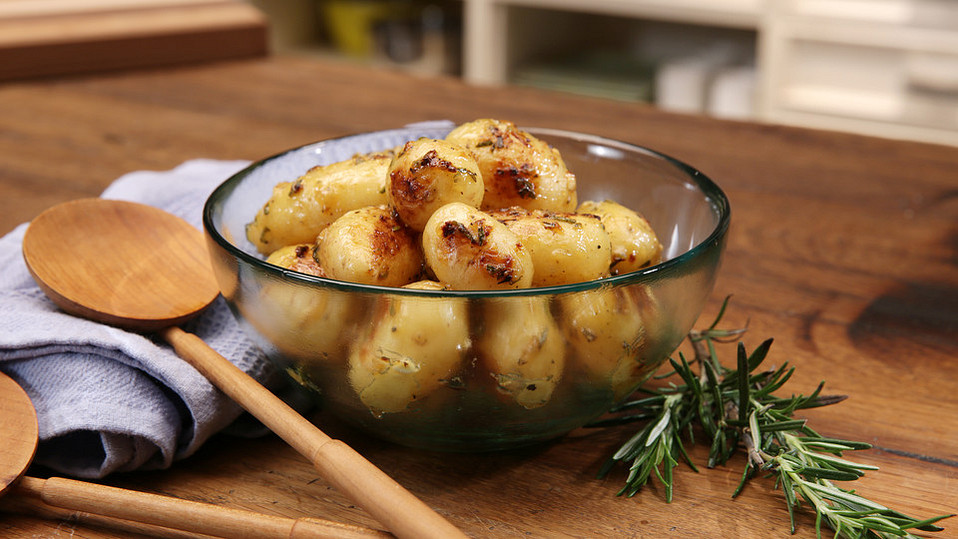
\includegraphics[width=.9\linewidth]{pics/Schwenkkartoffeln}
		\captionof{figure}{Schwenkkartoffeln von der Plancha}
		\label{fig:Schwenkkartoffeln}
	\end{minipage}
\end{figure}
\newpage

\subsection{Süßkartoffeln oder Kartoffeln aus der Folie}

\paragraph{Geräte}

\begin{itemize}[noitemsep]
	\item Kugelgrill oder Keramikgrill
\end{itemize}

\paragraph{Zutaten}
	
\begin{itemize}[noitemsep]
	\item Süßkartoffeln oder mehlig kochende Kartoffeln je nach Bedarf
\end{itemize}

\paragraph{Zubereitung}

Die Süßkartoffeln/ Kartoffeln in erst Backpapier und dann in Alu-Folie 
einwickeln.
Die Süßkartoffeln für ca. 45 Minuten die mehlig kochenden Kartoffeln evtl. kürzer 
direkt in die Glut legen. Nach 45 Minuten auspacken und servieren siehe 
Abbildungen~\vref{fig:Suess} ~\vref{fig:Folienkartoffel} Dazu wird ein Dip je nach Bedarf 
gereicht.
\newpage

\begin{figure}[htbp]
	\centering
	\begin{minipage}{1\textwidth}
		\centering
		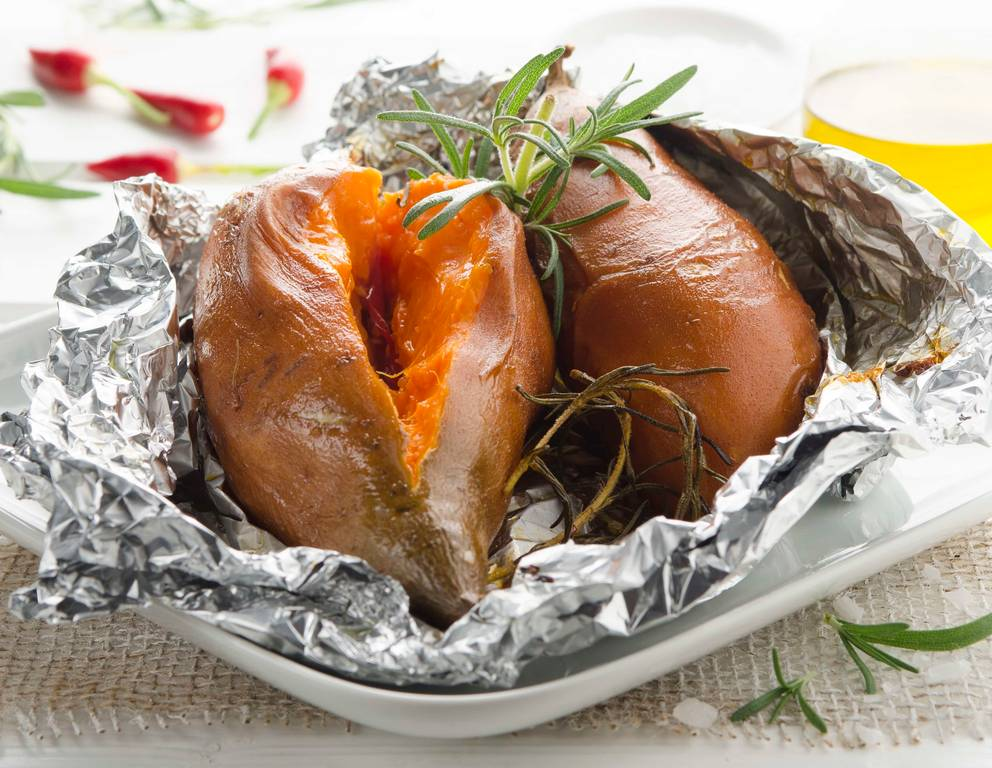
\includegraphics[width=.9\linewidth]{pics/Suess}
		\captionof{figure}{Foliensüßkartoffel vom Grill}
		\label{fig:Suess}
	\end{minipage}
\end{figure}

\begin{figure}[htbp]
	\centering
	\begin{minipage}{1\textwidth}
		\centering
		\includegraphics[width=1\linewidth]{pics/Folienkartoffel}
		\captionof{figure}{Folienkartoffel vom Grill}
		\label{fig:Folienkartoffel}
	\end{minipage}
\end{figure}
\newpage

